The full-system model of the Hyperloop can be decomposed into two main
subsystems: the passenger Pod and Tube. At the top level, these systems are
connected to basic cost estimation and notional
mission modules. \Cref{fig:top,fig:pod,fig:tube} below describe the structure of this model.
The appendix includes an eXtended Design Structure Matrix (XDSM) diagram key,
which describes how to interpret the following diagrams for the Pod, Tube, and Mission subsystems.

\begin{figure}
\centering
\begin{subfigure}[b]{.4\textwidth}
  \centering
  \centerline{\includegraphics[width=1.2\textwidth]{../images/tube_and_pod.png}}
  %\caption{Hierarchical tree}
  \label{fig:tree:tubeandpod}
\end{subfigure}%
\begin{subfigure}[b]{.6\textwidth}
  \centering
  \centerline{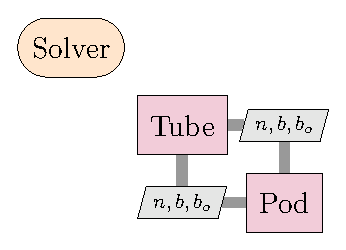
\includegraphics[width=1.4\textwidth,\vspace{1.2cm}]{../images/xdsm/tube_and_pod.pdf}}
  %\caption{XDSM}
  \label{fig:xdsm:toplevel}
\end{subfigure}
\caption{Top Level System Diagram, (Left) Hierarchical Tree, (Right) XDSM}
\label{fig:top}
\end{figure}

\begin{figure}
\centering
\begin{subfigure}[b]{.5\textwidth} % align [b]ottoms, 1cm padding on xdsm
  \centering
  \centerline{\includegraphics[width=1.3\textwidth]{../images/pod.png}}
  %\caption{Hierarchical tree}
  \label{fig:tree:pod}
\end{subfigure}%
\begin{subfigure}[b]{.5\textwidth}
  \centering
  \centerline{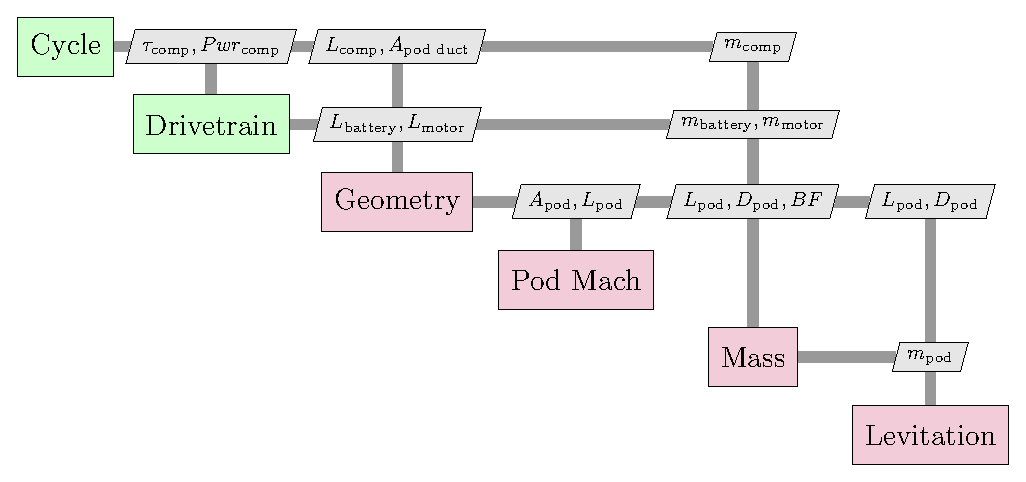
\includegraphics[width=1.4\textwidth,\vspace{0.5cm}]{../images/xdsm/pod.pdf}}
  %\caption{XDSM}
  \label{fig:xdsm:pod}
\end{subfigure}
\caption{Pod Assembly Diagram, (Left) Hierarchical Tree, (Right) XDSM}
\label{fig:pod}
\end{figure}

\begin{figure}[!]
\centering
\begin{subfigure}[b]{.5\textwidth} % align [b]ottoms, 1cm padding on xdsm
  \centering
  \centerline{\includegraphics[width=1.3\textwidth]{../images/tube.png}}
  %\caption{Hierarchical tree}
  \label{fig:tree:tube}
\end{subfigure}%
\begin{subfigure}[b]{.5\textwidth} % align [b]ottoms, 1cm padding on xdsm
  \centering
  \centerline{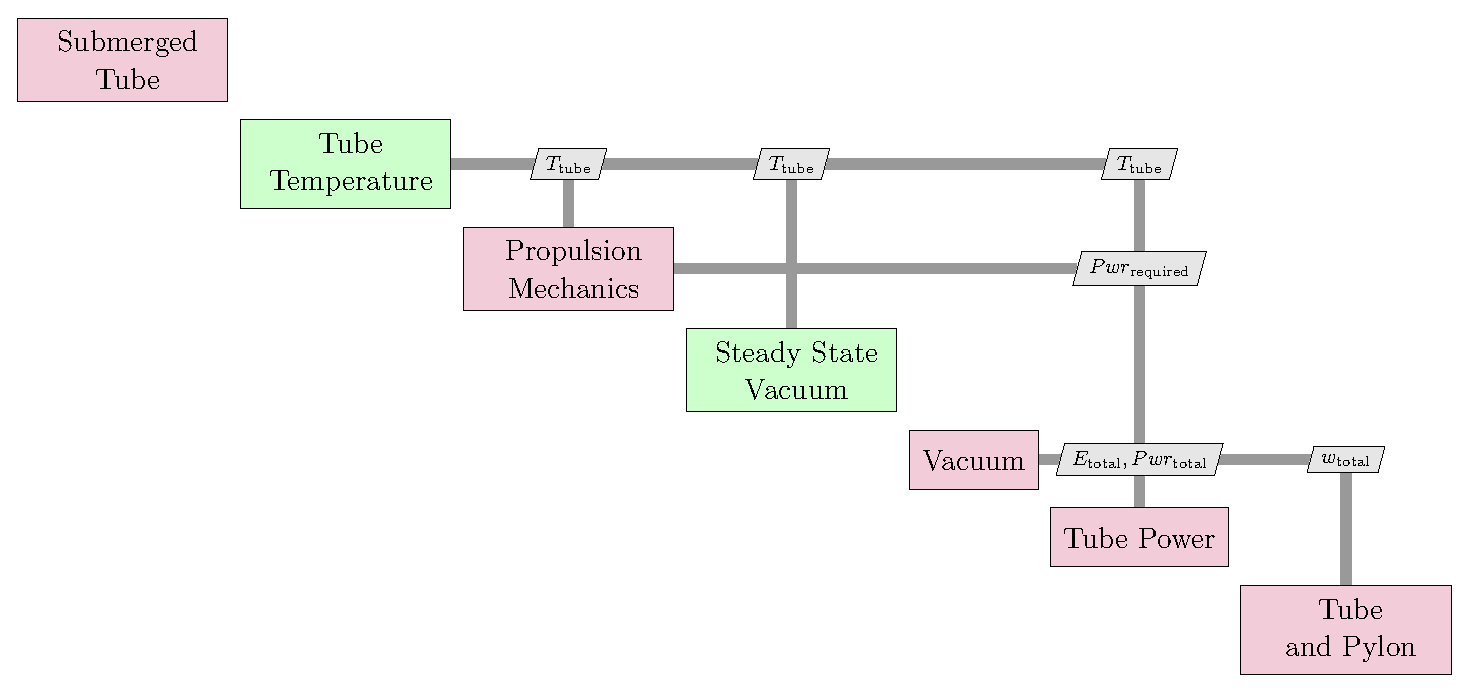
\includegraphics[width=1.3\textwidth,\vspace{0.8cm}]{../images/xdsm/tube.pdf}}
  %\caption{XDSM}
  \label{fig:xdsm:tube}
\end{subfigure}
\caption{Tube Assembly Diagram, (Left) Hierarchical Tree, (Right) XDSM}
\label{fig:tube}
\end{figure}


Additional levels of subsystems were broken down within the Pod and Tube assemblies.
Solver loops exist at multiple levels within the model, ensuring all design
constraints are satisfied across every subcomponent.
The XDSM diagrams indicates design variables that are passed from the output of
upstream components to be used as inputs for downstream components.
Further details can be found in following sections and in the source code
documentation, which is referenced in the Appendix.

\subsection{Top Level Component Descriptions}
	\subimport{model_overview/}{top_level_comp_descriptions}
\subsection{Pod Level Component Descriptions}
	\subimport{model_overview/}{pod_level_comp_descriptions}
\subsection{Tube Level Component Descriptions}
	\subimport{model_overview/}{tube_level_comp_descriptions}


